%==============================================================================
% TEMPLATE FOR THESIS WAGENINGEN UNIVERSITY
% CREATED BY AREND LIGTENBERG JUNE 2006;
% EDITED BY KIM CALDERS 2014;
% EDITED BY BEN DEVRIES 2015;
% EDITED BY LOIC DUTRIEUX 2016
%==============================================================================

\documentclass[10pt,twoside]{book}
\usepackage[T1]{fontenc}
% \usepackage{lmodern}
\usepackage[utf8]{inputenc}
\usepackage[dutch,english]{babel}
\usepackage{graphicx}
\usepackage{natbib}
\usepackage{bibentry} % bibentry for inserting complete BibTeX entries inline, explanation: http://stefaanlippens.net/bibentry
\nobibliography* % required by bibentry package;
\usepackage{amsmath}
\usepackage{fancyhdr}
\usepackage[small,bf]{caption}
%\captionsetup[table]{skip=10pt}
\usepackage{multirow}
\usepackage{threeparttable}
%\usepackage[body={6.0in, 8.2in},left=1.50in,right=1.50in]{geometry} %% very narrow
\usepackage[paperwidth=170mm, paperheight=240mm, margin=20mm]{geometry}
\usepackage[parfill]{parskip}
\usepackage{enumitem}
%\usepackage[rightcaption]{sidecap}
%\usepackage{epstopdf}
\usepackage{pdfpages}
\usepackage[hidelinks]{hyperref}
\usepackage{color}
\usepackage{xcolor}
\usepackage{colortbl}
\usepackage{appendix}

% extra packages added by Ben
\usepackage{rotating} % for rotating figures
\usepackage{changepage} % for indenting entire paragraphs
\usepackage{float} % help with table positioning
\floatstyle{plaintop} % caption on top
\restylefloat{table} % see above. Use: \begin{table}[H]
\usepackage{textcomp} % \textdegree
% \usepackage{fixltx2e} % for the \textsubscript command outside of a math environment. Removed by david, not required after 2015
\usepackage{csquotes} % for block quotes, use {displayquote} environment
\usepackage{todonotes}
\usepackage{soul}
\usepackage{fp}
\usepackage{tabularx}
\usepackage{subcaption}
\usepackage{pdflscape}
\usepackage{gensymb}
\usepackage[version=4]{mhchem}
\usepackage{wrapfig}

% Extra packages added by David
\usepackage{nomencl}
\usepackage{algorithm}
\usepackage[noend]{algpseudocode}
\usepackage{amssymb}
\usepackage{booktabs}
\usepackage{doi}
\usepackage{tikz} % for thumb tabs
\usepackage{lipsum} % for lorem ipsum text

\addto\captionsenglish{\renewcommand{\bibname}{References}}

\definecolor{Red}{rgb}{0.5,0,0}
\definecolor{Blue}{rgb}{0,0,0.5}


%=======================================================================
% GENERAL SETTINGS
%=======================================================================
%\oddsidemargin 40pt
%\evensidemargin 40pt
\setlength{\captionmargin}{5pt}
%\setlength{\textfloatsep}{10pt plus 1.0pt minus 2.0pt}
%\usepackage{pifont}
%\usepackage{times}
%\usepackage{txfonts}
\usepackage[sc]{mathpazo}
%\usepackage{setspace}

\linespread{1.1} %1 is single spacing, 1.3 is oneandhalf spacing


%\citationstyle{dcu}
\sloppy
\setcounter{tocdepth}{0}

%% for internal use
\newcommand{\fixme}[1]{\emph{\marginpar{FIXME} (#1)}}
\newcommand{\readme}[1]{\emph{\marginpar{README} (#1)}}
\newcommand{\verifyme}[1]{\emph{\marginpar{VERIFYME} (#1)}}


%=======================================================================
% THUMB TABS FOR CHAPTERS
%=======================================================================
% Chapter counter for thumb tab positioning
\newcounter{thumbchapter}
\setcounter{thumbchapter}{0}

% DEFINITION OF THE FANCY HEADERS
%=======================================================================
\pagestyle{fancy}
\renewcommand{\chaptermark}[1]{\markboth{#1}{}}
\renewcommand{\sectionmark}[1]{\markright{\thesection\ #1}}
\fancyhf{}
\fancyhead[LE,RO]{\bfseries\thepage}
\fancyhead[LO]{\bfseries\rightmark}
\fancyhead[RE]{\bfseries\leftmark}

% Add thumb tabs to headers
\fancyhead[RO]{%
  \bfseries\thepage%
  \ifnum\value{chapter}>0%
    \begin{tikzpicture}[remember picture, overlay]
      \node[
        fill=gray!80,
        text=white,
        font=\bfseries\normalsize,
        minimum height=1.0cm,
        minimum width=0.8cm,
        anchor=north east,
        rotate=0
      ] at ([xshift=0mm, yshift=-\value{thumbchapter}*1.8cm-2cm]current page.north east) {\thechapter};
    \end{tikzpicture}%
  \fi%
}
\fancyhead[LE]{%
  \bfseries\thepage%
  \ifnum\value{chapter}>0%
    \begin{tikzpicture}[remember picture, overlay]
      \node[
        fill=gray!80,
        text=white,
        font=\bfseries\normalsize,
        minimum height=1.0cm,
        minimum width=0.8cm,
        anchor=north west,
        rotate=0
      ] at ([xshift=0mm, yshift=-\value{thumbchapter}*1.8cm-2cm]current page.north west) {\thechapter};
    \end{tikzpicture}%
  \fi%
}

%=======================================================================
% NEW ENVIRONMENT FOR THE START OF CHAPTER (SMALL ABSTRACT)
%=======================================================================
\newenvironment{chapintro}
{
    \begin{center}
    \begin{minipage}[t]{0.9\textwidth}
    \hrule
    \medskip
    \small
}
{
    \medskip
    \hrule
    \end{minipage}
    \end{center}
    \bigskip
}


%=======================================================================
% ADD WORD CHAPTER FOR TOC
%=======================================================================


\makeatletter
\let\orig@chapter\@chapter
\def\@chapter[#1]#2{\ifnum \c@secnumdepth >\m@ne
                       \if@mainmatter
                         \refstepcounter{chapter}%
                         \typeout{\@chapapp\space\thechapter.}%
                         \addcontentsline{toc}{chapter}%
                                   {Chapter~\protect\numberline{\thechapter}#1}%
                       \else
                         \addcontentsline{toc}{chapter}{#1}%
                       \fi
                    \else
                      \addcontentsline{toc}{chapter}{#1}%
                    \fi
                    \chaptermark{#1}%
                    \addtocontents{lof}{\protect\addvspace{10\p@}}%
                    \addtocontents{lot}{\protect\addvspace{10\p@}}%
                    \if@twocolumn
                      \@topnewpage[\@makechapterhead{#2}]%
                    \else
                      \@makechapterhead{#2}%
                      \@afterheading
                    \fi}
\makeatother

%=======================================================================
% CUSTOM CHAPTER HEAD FORMATTING - REDUCE TOP SPACING
%=======================================================================
\makeatletter
\def\@makechapterhead#1{%
  \vspace*{15\p@}%  % Negative spacing to move chapter titles up by ~1.5cm
  {\parindent \z@ \raggedright \normalfont
    \ifnum \c@secnumdepth >\m@ne
      \if@mainmatter
        \huge\bfseries \@chapapp\space \thechapter
        \par\nobreak
        \vskip 20\p@
      \fi
    \fi
    \interlinepenalty\@M
    \Huge \bfseries #1\par\nobreak
    \vskip 40\p@
  }}
\makeatother

%=======================================================================
% CUSTOM UNNUMBERED CHAPTER HEAD FORMATTING (for Contents, etc.)
%=======================================================================
\makeatletter
\def\@makeschapterhead#1{%
  \vspace*{-15\p@}%  % Same negative spacing for unnumbered chapters
  {\parindent \z@ \raggedright
    \normalfont
    \interlinepenalty\@M
    \Huge \bfseries #1\par\nobreak
    \vskip 40\p@
  }}
\makeatother

%=======================================================================
% A BIT MORE COMPACT ITEM LIST
%=======================================================================
\newenvironment{itemize*}%
  {\begin{itemize}%
    \setlength{\parskip}{0pt}%
    \setlength{\itemsep}{0pt}%
    \setlength{\parsep}{0pt}}%
  {\end{itemize}}

%more compact enumeration list
  \newenvironment{enumerate*}%
  {\begin{enumerate}%
    \setlength{\itemsep}{0pt}%
    \setlength{\parskip}{0pt}}%
  {\end{enumerate}}

%=======================================================================
% A BIT MORE COMPACT DESCRIPTION LIST
%=======================================================================
\renewcommand{\descriptionlabel}[1]{\hspace{\labelsep}\textrm{#1}}

\newenvironment{description*}%
  {\begin{description}%
    \setlength{\itemsep}{0pt}%
    \setlength{\parskip}{0pt}}%
  {\end{description}}

%=======================================================================
% A BIT MORE COMPACT BIBLIOGRAPHY
%=======================================================================
  \let\oldthebibliography=\thebibliography
  \let\endoldthebibliography=\endthebibliography
  \renewenvironment{thebibliography}[1]{%
    \begin{oldthebibliography}{#1}%
      \setlength{\parskip}{0ex}%
      \setlength{\itemsep}{1ex}%
  }%
  {%
    \end{oldthebibliography}%
  }

%=======================================================================
% CLEAR HEADER STYLE ON LAST EMPTY ODD PAGES
%=======================================================================
\makeatletter
\def\cleardoublepage{\clearpage\if@twoside \ifodd\c@page\else%
\hbox{}%
\thispagestyle{empty}%
\newpage%
\if@twocolumn\hbox{}\newpage\fi\fi\fi}
\makeatother


%=======================================================================
% SOME EXTRA COMMANDS FOR VISUAL LAYOUT
%=======================================================================
\newcommand{\longpage}{\enlargethispage{\baselineskip}}
\newcommand{\shortpage}{\enlargethispage{-\baselineskip}}
\newcommand{\setreference}{\vspace*{\fill}}

%=======================================================================
% LIST ENVIRONMENT FOR OWN SELECTED PUBLICATIONS
%=======================================================================
\newenvironment{pubs}
{
\begin{list}{}
{%
\item[]}%
\setlength{\itemindent}{-25pt}%
\setlength{\parsep}{-0pt}
\setlength{\itemsep}{-0pt}
}%
{\end{list}%
}%


%==============================
% REFORMAT SECTION HEADINGS
%==============================

%% using titlesec
\usepackage{titlesec}
%% FIX FOR BUG in titlesec 2.10.1
\usepackage{etoolbox}

\makeatletter
\patchcmd{\ttlh@hang}{\parindent\z@}{\parindent\z@\leavevmode}{}{}
\patchcmd{\ttlh@hang}{\noindent}{}{}{}
\makeatother
%% END OF BUGFIX

\titleformat{\subsection}
  {\normalfont\normalsize\bfseries}
  {\thesubsection}{1em}{}
\titleformat{\subsubsection}
  {\normalfont\normalsize\itshape}
  {\thesubsubsection}{1em}{}



%==============================
% Force start of newpage on left page
%==============================
\newcommand*\cleartoleftpage{%
  \clearpage
  \ifodd\value{page}\hbox{}\newpage\fi
}



%=======================================================================
% INCLUSION OF THE CONTENT
%=======================================================================

\raggedbottom % preferentially leaves whitespace at bottom of page instead of distributing throughout vertical space

\begin{document}

\frontmatter
\pagenumbering{alph}
\pagenumbering{roman}
\addtocontents{toc}{~\hfill\rlap{\textbf{Page}}\par}
\thispagestyle{empty}
%%%%%%%%%%%%%%%%%%%%%%%%%%%%%%%%%%%%%%%%%%%%%%%%%%%%%%%%%%%%%%%%%%
\begin{center}
\Huge{\textbf{Your PhD thesis title}} \\
% \Huge{\textbf{Thesis}} \\
\vspace*{1cm}
\vspace*{1cm}
\vspace*{\fill}
\large{David Q. Researcher}\\
\end{center}

%%%%%%%%%%%%%%%%%%%%%%%%%%%%%%%%%%%%%%%%%%%%%%%%%%%%%%%%%%%%%%%%
\newpage
\thispagestyle{empty}
\vspace*{\fill}
\begin{tabular}{l}
    \textbf{Thesis committee}                                                                 \\  
                                                                                              \\  
    	extbf{Promotor:}                                                                        \\
    Prof. Dr. A.B. Example                                                                 \\
    Professor of Example Discipline                                                   \\
    Example University \& Research Institute                                                   \\
                                                                                              \\  
    	extbf{Co-promotors:}                                                                    \\
    Dr. C.D. Sample                                                                    \\
    Associate Professor, Example Discipline                             \\
    Example University \& Research Institute                                           \\
                                                                                              \\  

    	extbf{Other members:}                                                                   \\
    Prof. Dr. E.F. Reviewer, Example University \& Research          \\
    Prof. Dr. G.H. Scientist, Example University of Technology                   \\
    Prof. Dr. I.J. Academic, International Example University                                   \\
    Dr. K.L. Expert, Example University \& Research                                  \\
    \\  

    \small{This research was conducted under the auspices of the Graduate School} \\  
    \small{of Production Ecology \& Resource Conservation (PE$\&$RC)}                         \\  
\end{tabular}

%%%%%%%%%%%%%%%%%%%%%%%%%%%%%%%%%%%%%%%%%%%%%%%%%%%%%%%%%%%%%%%%
\newpage
\thispagestyle{empty}
\begin{center}
\Huge{\textbf{Your PhD thesis title}} \\
% \Huge{\textbf{thesis}} \\
\vspace*{1cm}
\Large{David Q. Researcher}\\
\normalsize
\vspace*{\fill}
\textbf{Thesis} \\
submitted in fulfilment of the requirements for the degree of doctor at \\
Wageningen University\\
by the authority of the Rector Magnificus\\
Prof. Dr C. Kroeze,\\
in the presence of the\\
Thesis Committee appointed by the Academic Board\\
to be defended in public\\
on Wednesday 19 November 2025\\
at 1 p.m. in the Omnia Auditorium.\\
\end{center}

%%%%%%%%%%%%%%%%%%%%%%%%%%%%%%%%%%%%%%%%%%%%%%%%%%%%%%%%%%%%%%%%%%%
\newpage
\thispagestyle{empty}
\vspace*{\fill}
\begin{flushleft}
\begin{tabular}{l}
    David Q. Researcher                                                 \\  
    Your PhD thesis title                                     \\  
    148 pages.                                               \\  
                                                             \\  
    PhD thesis, Wageningen University \& Research, Wageningen, NL (2025) \\  
    With references, with summary in English and Spanish     \\  
                                                             \\  
    DOI https://doi.org/10.18174/681245                                             \\  
\end{tabular}
\end{flushleft}
%\newpage
%\thispagestyle{empty}
%\begin{flushright}
%\vspace*{\fill}
%\textit{Aan mijn ouders}
%\end{flushright}

\cleardoublepage
\cleardoublepage
\phantomsection

\chapter{Summary}
\label{cha:Summary}

\lipsum[1-3]
\cleardoublepage
\phantomsection

\addcontentsline{toc}{chapter}{Contents}  
\tableofcontents
\cleardoublepage
\phantomsection
\pagenumbering{arabic} \setcounter{page}{1}


%% Main Chapters
\mainmatter
\setcounter{page}{1}
\setcounter{thumbchapter}{1}\chapter[Introduction]{Introduction}
\chaptermark{Introduction}
\label{cha:chapter1}
\vspace*{\fill}


\newpage

\section{Wageningen University \& Research (WUR) template}
Wageningen University \& Research (WUR) is a renowned institution specializing in life sciences, agricultural research, and environmental studies. The university is located in Wageningen, Netherlands, and is known for its strong emphasis on sustainability, food security, and innovative agricultural practices. WUR collaborates with various international organizations, governments, and industries to address global challenges related to food production, climate change, and natural resource management. One of the main buildings of WUR is the Forum building, which serves as a central hub for students. You can see a picture of the Forum building in Figure \ref{fig:forum_wur_building}.

Your text with citations one way \cite{example_author_example_2024} or another \citep{example_author_example_2024}.


\begin{figure}[!ht]
    \centering
    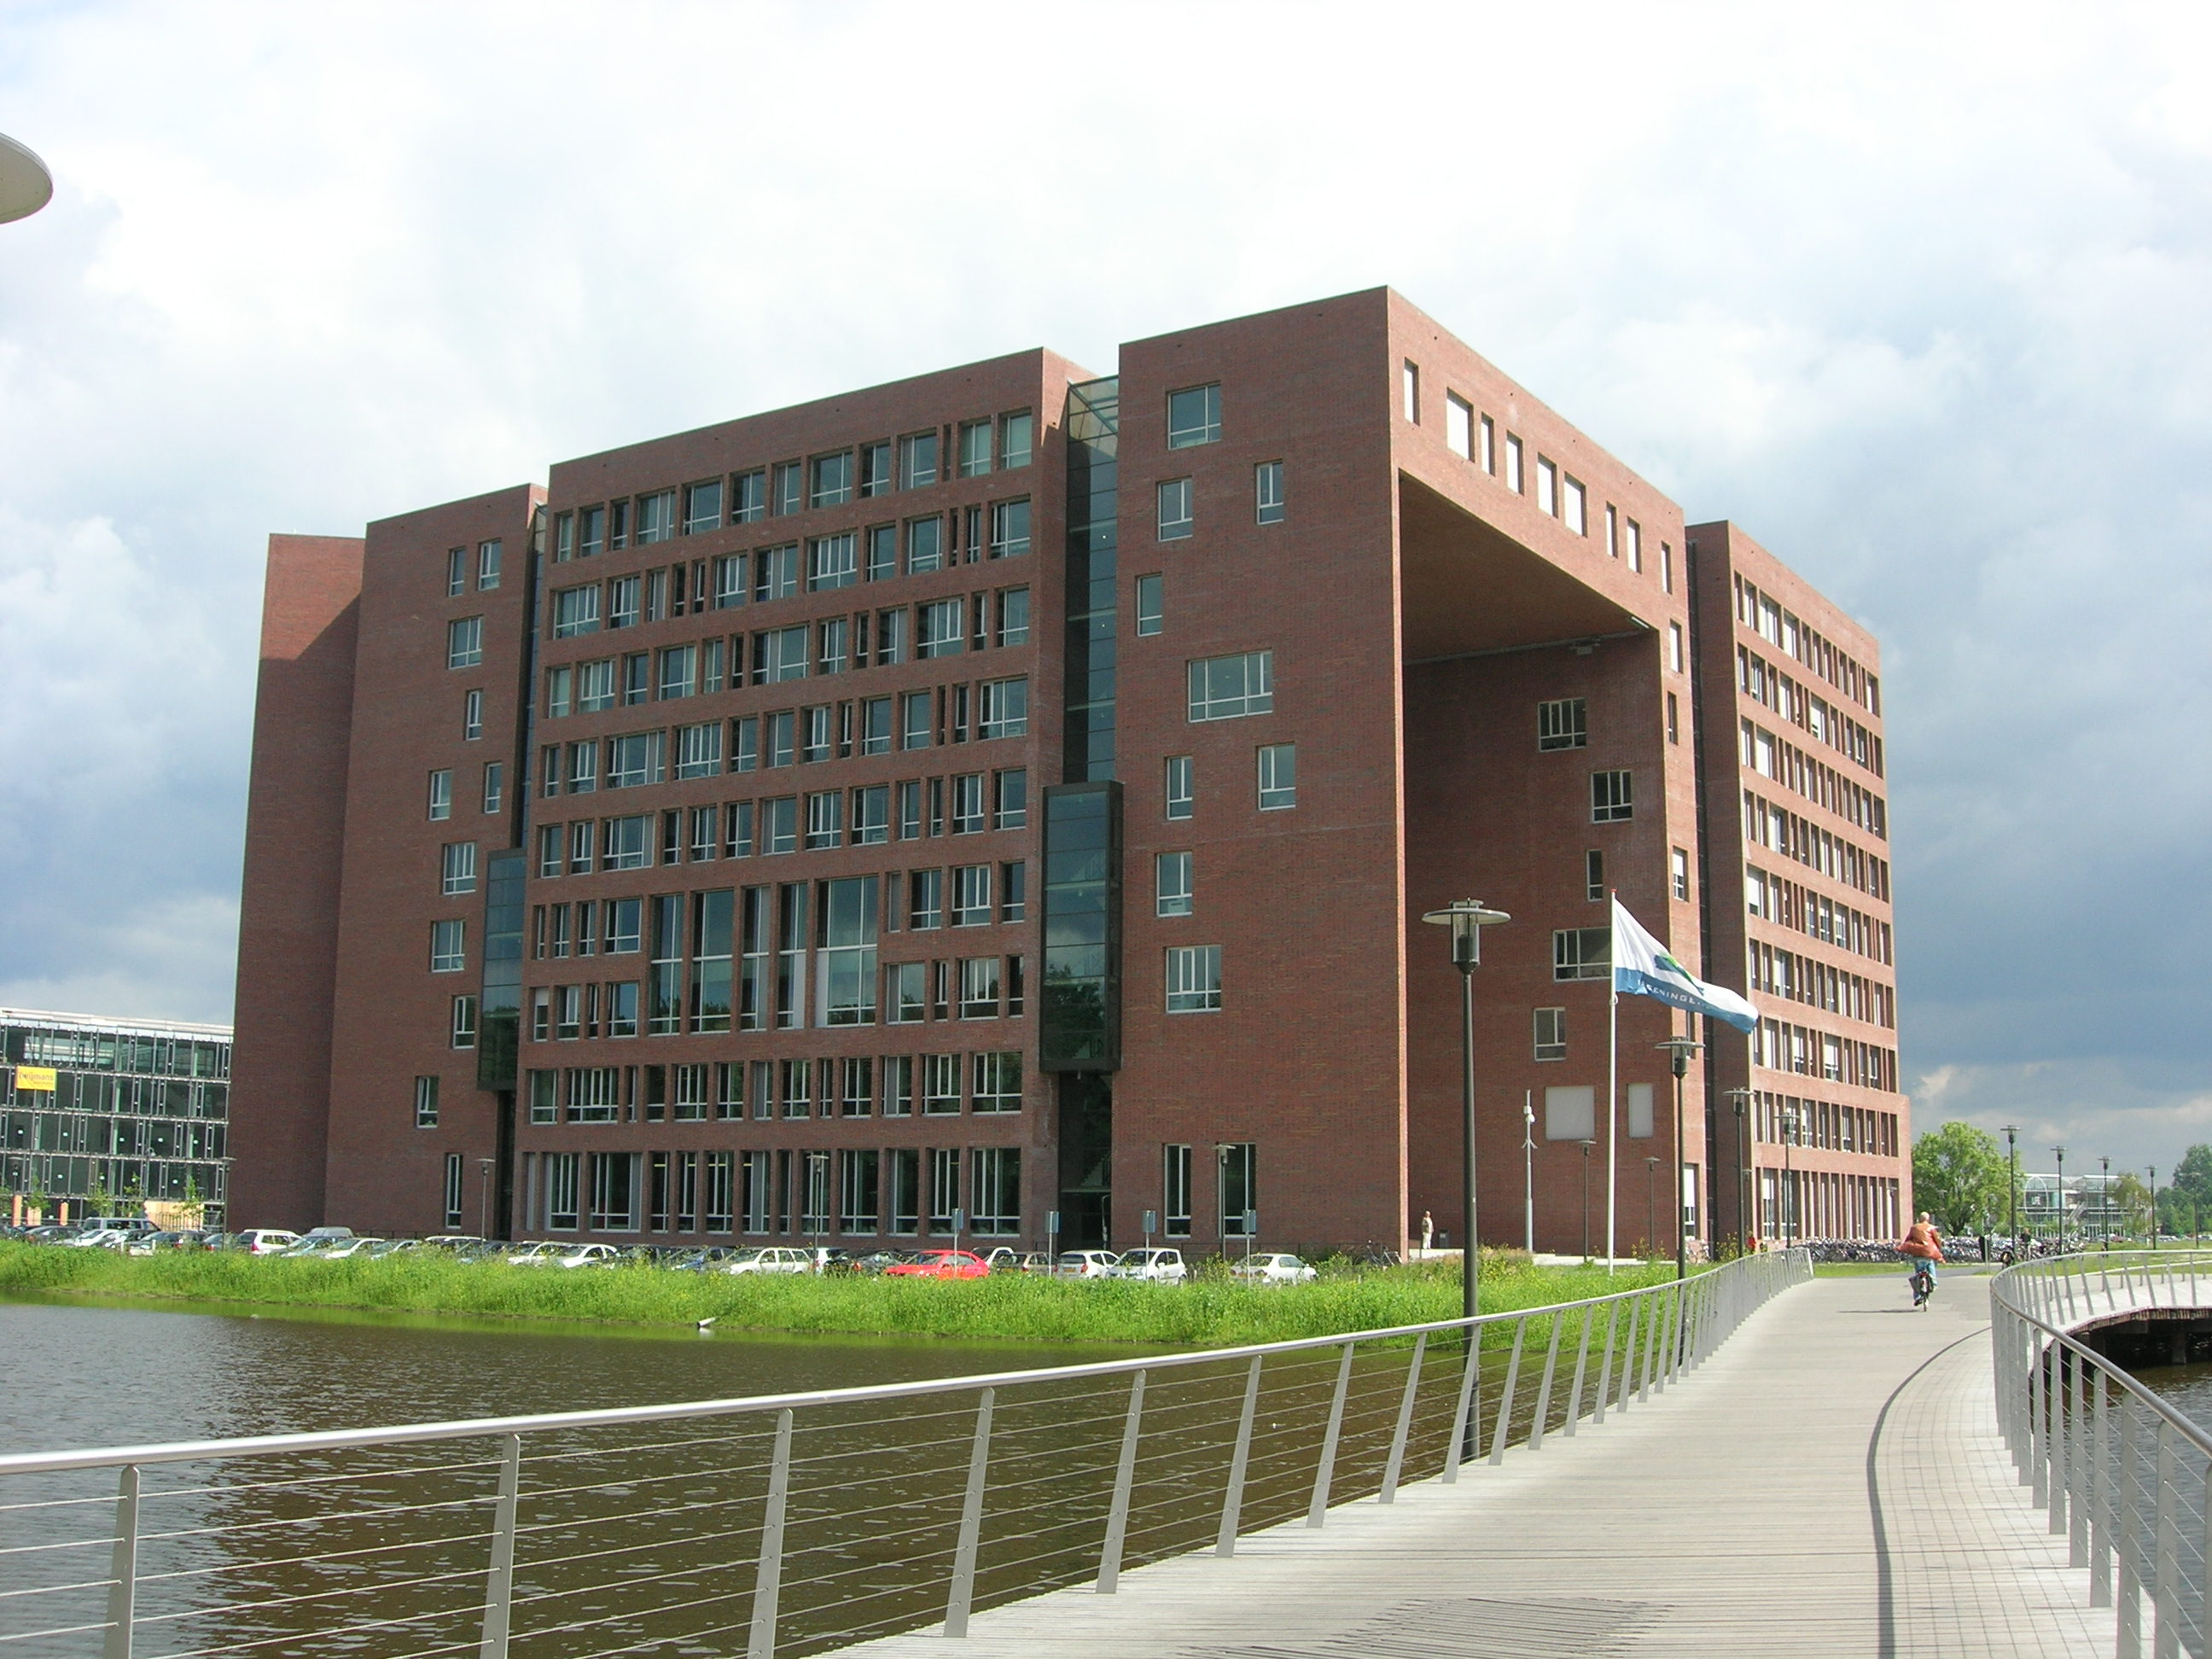
\includegraphics[width=0.75\linewidth]{assets/ch1/WUR_forum_building.jpg}
    \caption{A picture of the Forum building at Wageningen University \& Research.}
    \label{fig:forum_wur_building}
\end{figure}

\lipsum[1-5]      % Generates first 5 paragraphs

\section{Thesis overview}

\lipsum[6] % Introduction 
\stepcounter{thumbchapter}\chapter[Example study on multi-view perception and 3D object tracking in controlled environments]{Example study on multi-view perception and 3D object tracking in controlled environments}
\chaptermark{Example multi-view 3D tracking system}
\label{cha:chapter2}
\vspace*{\fill}
\textbf{This chapter is based on:}

David Q. Researcher, A. B. Coauthor, \& C. D. Collaborator (2023). Example study on multi-view perception and 3D object tracking in controlled environments. \textit{Example Journal}, 231, 78-91.
\newpage
\newpage

\section*{Abstract}
\lipsum[1]

\newpage

\section{Introduction}

\lipsum[1-3]

\section{Conclusions and future work} 
\lipsum[4]
\stepcounter{thumbchapter}\chapter[Example sparse convolution feature extractor for improving 3D multi-object tracking]{Example sparse convolution feature extractor for improving 3D multi-object tracking}
\chaptermark{Example sparse feature extractor for MOT}
\label{cha:chapter3}
\vspace*{\fill}
\textbf{This chapter is based on:}

David Q. Researcher, A. B. Coauthor, \& C. D. Collaborator (2023). Example sparse convolution feature extractor for improving 3D multi-object tracking. \textit{Example Journal}, 236, 193-200.
\newpage

\section*{Abstract}
\lipsum[1]

\newpage

\section{Introduction}

\lipsum[1-3]

\section{Conclusions and future work} 
\lipsum[4]
\stepcounter{thumbchapter}\chapter[Example transformer-based single-shot 3D detection and tracking approach]{Example transformer-based single-shot 3D detection and tracking approach}
\chaptermark{Example transformer 3D detection and tracking}
\label{cha:chapter4}
\vspace*{\fill}
\textbf{This chapter is based on:}

David Q. Researcher, E. F. Teammate, G. H. Contributor, I. J. Senior, \& K. L. Advisor (2024). Example transformer-based single-shot 3D detection and tracking approach. \textit{Example Journal}, 225, 109275.
\newpage

\section*{Abstract}
\lipsum[1]

\newpage

\section{Introduction}

\lipsum[1-3]

\section{Conclusions and future work} 
\lipsum[4]
\stepcounter{thumbchapter}\chapter[Example comparison between single-stage and two-stage 3D tracking algorithms]{Example comparison between single-stage and two-stage 3D tracking algorithms}
\chaptermark{Example comparison of tracking paradigms}
\label{cha:chapter5}
\vspace*{\fill}
\textbf{This chapter is based on:}

David Q. Researcher, M. N. Analyst, O. P. Advisor, \& Q. R. Mentor (2024). Example comparison between single-stage and two-stage 3D tracking algorithms. \textit{Example Journal}, 24(22), 7332.
\newpage

\section*{Abstract}
\lipsum[1]

\newpage

\section{Introduction}

\lipsum[1-3]

\section{Conclusions and future work} 
\lipsum[4]
\stepcounter{thumbchapter}\include{06_chapter6} % Discussion


\backmatter
\bibliographystyle{model5-names}
\phantomsection
\addcontentsline{toc}{chapter}{References}
\bibliography{references}
\fancyhead{}

\cleardoublepage
\phantomsection

\addcontentsline{toc}{chapter}{Acknowledgements}
\chapter*{Acknowledgements}

I would like to express my gratitude to all those who have supported me along the way. Without their help, this thesis would not have been possible.

\lipsum[1]
\cleardoublepage
\phantomsection

%% Back Matter
\phantomsection
\chapter{About the author}
% Replace the lipsum below with a short professional biography of the author.
% Suggested contents: background, education, research interests, key achievements.
\lipsum[1-2]

\section*{Peer-reviewed journal publications}
% Provide publications in reverse chronological order. Follow a consistent citation style.
% TEMPLATE FORMAT:
% Surname, I. I., Surname, I. I., & Surname, I. I. (Year). Title of the article in sentence case: Subtitle if needed. \textit{Journal Name}, Volume(Issue), page–page. doi:DOI

Author, A. A., Researcher, B. B., \& Collaborator, C. C. (2025). Example article demonstrating multi-view plant analysis using integrated sensing. \textit{Journal of Example Robotics}, 42(3), 101–119. doi:10.0000/jer.2025.000001.

Author, A. A., \& Teammate, D. D. (2024). Sparse feature fusion for efficient 3D object tracking in controlled agriculture environments. \textit{International Journal of Applied Vision}, 18(2), 55–73. doi:10.0000/ijav.2024.000002.

Author, A. A., Expert, E. E., Analyst, F. F., \& Advisor, G. G. (2023). Unified transformer framework for single-shot detection and tracking in structured canopies. \textit{Computational Sensing Letters}, 7(1), 1–14. doi:10.0000/csl.2023.000003.

\section*{Conference proceedings}
% TEMPLATE FORMAT:
% Surname, I. I., Surname, I. I., & Surname, I. I. (Year, Month). Title in sentence case. In \textit{Proceedings of the Full Conference Name (ACRONYM)} (pp. xxx–xxx). Publisher. doi:DOI (if available)

Presenter, H. H., Coauthor, I. I., \& Mentor, J. J. (2025, September). Real-time multi-sensor fusion for adaptive canopy yield estimation. In \textit{Proceedings of the IEEE International Conference on Agricultural Automation (ICAA)} (pp. 210–217). IEEE. doi:10.0000/icaa.2025.000021.

Engineer, K. K., Author, A. A., \& Developer, L. L. (2024, June). Lightweight transformer kernels for embedded 3D tracking. In \textit{Proceedings of the International Conference on Field Robotics (ICFR)} (pp. 88–95). ACM. doi:10.0000/icfr.2024.000045.

\section*{Conference workshop contributions}
% TEMPLATE FORMAT:
% Surname, I. I., Surname, I. I., & Surname, I. I. (Year). Title in sentence case. Poster (or Oral) presented at the Workshop on Title, Conference Name (ACRONYM), City, Country.

Author, A. A., Collaborator, C. C., \& Advisor, D. D. (2025). Comparative evaluation of single-stage and two-stage 3D tracking paradigms in dense foliage. Poster presented at the Workshop on Field Robotics, International Conference on Robotics and Automation (ICRA), Barcelona, Spain.

Researcher, E. E., \& Scientist, F. F. (2024). Self-supervised feature bootstrapping for plant-scale reconstruction. Oral presentation at the Workshop on Emerging Methods in Agricultural Vision, European Conference on Computer Vision (ECCV), Milan, Italy.

\section*{Preprint (not peer-reviewed)}
% TEMPLATE FORMAT:
% Surname, I. I., & Surname, I. I. (Year). Title in sentence case. \textit{arXiv preprint} arXiv:xxxx.xxxxx. doi:DOI (if assigned)

Author, A. A., \& Collaborator, B. B. (2025). Orchard-SLAM: Semantic-aware simultaneous localization and mapping for structured perennial crops. \textit{arXiv preprint} arXiv:2501.01234. doi:10.0000/arxiv.2501.01234.

Researcher, C. C. (2024). Multi-modal transformer encoders for sparse agricultural scene understanding. \textit{arXiv preprint} arXiv:2412.09876.
\cleardoublepage
\phantomsection

\chapter{PE\&RC Training and Education Statement}

\begin{minipage}[c]{.55\textwidth}

With the training and education activities listed below the PhD candidate has complied with the requirements set by the Graduate School for Production Ecology and Resource Conservation (PE\&RC) which comprises of a minimum total of 30 ECTS (= 20 weeks of activities) 
\end{minipage}
\begin{minipage}[c]{.35\textwidth}
\begin{flushright}
\vspace{0pt}
\includegraphics[width=4.6cm,height=4.6cm]{PERC_logo.pdf}
\end{flushright}
\end{minipage}

\bigskip

\textbf{Writing of project proposal (4.5 ECTS)}
\begin{itemize}[nolistsep]
    \item [Your project proposal title]
\end{itemize}

\textbf{Post-graduate courses (4 ECTS)}
\begin{itemize}[nolistsep]
    \item Course Name, Institution (Year)
    \item Course Name, Institution (Year)
\end{itemize}

\textbf{Invited review of (unpublished) journal manuscript (6 ECTS)}
\begin{itemize}[nolistsep]
    \item Journal Name: Article Title (Year)
    \item Journal Name: Article Title (Year)
    \item Journal Name: Article Title (Year)
    \item Journal Name: Article Title (Year)
    \item Journal Name: Article Title (Year)
\end{itemize}

\textbf{Competence, Skills and Career-oriented activities (2.7 ECTS)}
\begin{itemize}[nolistsep]
    \item Course/Workshop Name; Institution (Year)
    \item Course/Workshop Name; Institution (Year)
    \item Course/Workshop Name; Institution (Year)
\end{itemize}

\textbf{Scientific Integrity/Ethics in science activities (0.6 ECTS)}
\begin{itemize}[nolistsep]
    \item Course Name; Institution (Year)
\end{itemize}

\textbf{PE\&RC Retreat, PE\&RC Day, and other PE\&RC events (1.2 ECTS)}
\begin{itemize}[nolistsep]
    \item Event Name (Year)
    \item Event Name (Year)
\end{itemize}

\textbf{National / local scientific meetings, seminars, and discussion groups (6.5 ECTS)}
\begin{itemize}[nolistsep]
    \item Meeting/Event Name; Location (Year--Year)
    \item Meeting/Event Name; Location (Year--Year)
\end{itemize}

\textbf{International symposia, workshops and conferences (5.4 ECTS)}
\begin{itemize}[nolistsep]
    \item Conference Name; Location (Year)
    \item Conference Name; Location (Year)
    \item Conference Name; Location (Year)
\end{itemize}

\textbf{Societally relevant exposure (0.3 ECTS)}
\begin{itemize}[nolistsep]
    \item Event/Activity Name (Year)
\end{itemize}

\textbf{Lecturing / supervision of practical’s / tutorials (18 ECTS)}
\begin{itemize}[nolistsep]
    \item (Course code) Course name (Year)
    \item (Course code) Course name (Year--Year) % for multi-year courses
\end{itemize}

\textbf{BSc / MSc thesis supervision (3 ECTS)}
\begin{itemize}[nolistsep]
    \item Thesis Title 1
    \item Thesis Title 2
    \item Thesis Title 3
    \item Thesis Title 4
    \item Thesis Title 5
    \item Thesis Title 6
\end{itemize}


\renewcommand{\headrulewidth}{0pt}
\cleartoleftpage

\chapter*{Authorship statement}
\phantomsection
\addcontentsline{toc}{chapter}{Authorship statement}

\textit{Chapter 1: Introduction} \\
\lipsum[1]
\vspace{1em}

\textit{Chapter 2: ...} \\
\lipsum[2]
\vspace{1em}

\textit{Chapter 3: ...} \\
\lipsum[3]
\vspace{1em}

\textit{Chapter 4: ...} \\
\lipsum[4]
\vspace{1em}

\textit{Chapter 5: ...} \\
\lipsum[5]
\vspace{1em}

\textit{Chapter 6: General discussion} \\
\lipsum[6]
\cleartoleftpage

\vspace*{1cm}
This research received funding from Project XXX.

\vspace*{\fill}
Cover design by Designer Name.
\end{document}